%----------
%	CONFIGURACIÓN DEL DOCUMENTO
%----------

% Definimos las características del documento y añadimos una serie de paquetes (\usepackage{package}) que agregan funcionalidades a LaTeX.

\documentclass[12pt]{report} %fuente a 12pt

% MÁRGENES: 2,5 cm sup. e inf.; 3 cm izdo. y dcho.
\usepackage[
a4paper,
vmargin=2.5cm,
hmargin=3cm
]{geometry}

% INTERLINEADO: Estrecho (6 ptos./interlineado 1,15) o Moderado (6 ptos./interlineado 1,5)
\renewcommand{\baselinestretch}{1.15}
\parskip=6pt

% DEFINICIÓN DE COLORES para portada y listados de código
\usepackage[table]{xcolor}
\definecolor{azulUC3M}{RGB}{0,0,102}
\definecolor{gray97}{gray}{.97}
\definecolor{gray75}{gray}{.75}
\definecolor{gray45}{gray}{.45}

% Soporte para GENERAR PDF/A --es importante de cara a su inclusión en e-Archivo porque es el formato óptimo de preservación y a la generación de metadatos, tal y como se describe en http://uc3m.libguides.com/ld.php?content_id=31389625. En la carpeta incluímos el archivo plantilla_tfg_2017.xmpdata en el que puedes incluir los metadatos que se incorporarán al archivo PDF cuando lo compiles. Ese archivo debe llamarse igual que tu archivo .tex. Puedes ver un ejemplo en esta misma carpeta.
\usepackage[a-1b]{pdfx}

% ENLACES
\usepackage{hyperref}
\hypersetup{colorlinks=true,
	linkcolor=black, % enlaces a partes del documento (p.e. índice) en color negro
	urlcolor=blue} % enlaces a recursos fuera del documento en azul

% EXPRESIONES MATEMATICAS
\usepackage{amsmath,amssymb,amsfonts,amsthm}

\usepackage{txfonts} 
\usepackage[T1]{fontenc}
\usepackage[utf8]{inputenc}

\usepackage[spanish, es-tabla]{babel} 
\usepackage[babel, spanish=spanish]{csquotes}
\AtBeginEnvironment{quote}{\small}

% diseño de PIE DE PÁGINA
\usepackage{fancyhdr}
\pagestyle{fancy}
\fancyhf{}
\renewcommand{\headrulewidth}{0pt}
\rfoot{\thepage}
\fancypagestyle{plain}{\pagestyle{fancy}}

% DISEÑO DE LOS TÍTULOS de las partes del trabajo (capítulos y epígrafes o subcapítulos)
\usepackage{titlesec}
\usepackage{titletoc}
\titleformat{\chapter}[block]
{\large\bfseries\filcenter}
{\thechapter.}
{5pt}
{\MakeUppercase}
{}
\titlespacing{\chapter}{0pt}{0pt}{*3}
\titlecontents{chapter}
[0pt]                                               
{}
{\contentsmargin{0pt}\thecontentslabel.\enspace\uppercase}
{\contentsmargin{0pt}\uppercase}                        
{\titlerule*[.7pc]{.}\contentspage}                 

\titleformat{\section}
{\bfseries}
{\thesection.}
{5pt}
{}
\titlecontents{section}
[5pt]                                               
{}
{\contentsmargin{0pt}\thecontentslabel.\enspace}
{\contentsmargin{0pt}}
{\titlerule*[.7pc]{.}\contentspage}

\titleformat{\subsection}
{\normalsize\bfseries}
{\thesubsection.}
{5pt}
{}
\titlecontents{subsection}
[10pt]                                               
{}
{\contentsmargin{0pt}                          
	\thecontentslabel.\enspace}
{\contentsmargin{0pt}}                        
{\titlerule*[.7pc]{.}\contentspage}  


% DISEÑO DE TABLAS. Puedes elegir entre el estilo para ingeniería o para ciencias sociales y humanidades. Por defecto, está activado el estilo de ingeniería. Si deseas utilizar el otro, comenta las líneas del diseño de ingeniería y descomenta las del diseño de ciencias sociales y humanidades
\usepackage{multirow} % permite combinar celdas 
\usepackage{caption} % para personalizar el título de tablas y figuras
\usepackage{floatrow} % utilizamos este paquete y sus macros \ttabbox y \ffigbox para alinear los nombres de tablas y figuras de acuerdo con el estilo definido. Para su uso ver archivo de ejemplo 
\usepackage{array} % con este paquete podemos definir en la siguiente línea un nuevo tipo de columna para tablas: ancho personalizado y contenido centrado
\newcolumntype{P}[1]{>{\centering\arraybackslash}p{#1}}
\DeclareCaptionFormat{upper}{#1#2\uppercase{#3}\par}

% Diseño de tabla para ingeniería
\captionsetup[table]{
	format=upper,
	name=TABLA,
	justification=centering,
	labelsep=period,
	width=.75\linewidth,
	labelfont=small,
	font=small,
}

%Diseño de tabla para ciencias sociales y humanidades
%\captionsetup[table]{
%	justification=raggedright,
%	labelsep=period,
%	labelfont=small,
%	singlelinecheck=false,
%	font={small,bf}
%}


% DISEÑO DE FIGURAS. Puedes elegir entre el estilo para ingeniería o para ciencias sociales y humanidades. Por defecto, está activado el estilo de ingeniería. Si deseas utilizar el otro, comenta las líneas del diseño de ingeniería y descomenta las del diseño de ciencias sociales y humanidades
\usepackage{graphicx}
\graphicspath{{res/}} %ruta a la carpeta de imágenes

\usepackage{afterpage}
% Diseño de figuras para ingeniería
\captionsetup[figure]{
	format=hang,
	name=Fig.,
	singlelinecheck=off,
	labelsep=period,
	labelfont=small,
	font=small		
}


% NOTAS A PIE DE PÁGINA
\usepackage{chngcntr} %para numeración contínua de las notas al pie
\counterwithout{footnote}{chapter}

% LISTADOS DE CÓDIGO
% soporte y estilo para listados de código. Más información en https://es.wikibooks.org/wiki/Manual_de_LaTeX/Listados_de_código/Listados_con_listings
\usepackage{listings}

% definimos un estilo de listings
\lstdefinestyle{estilo}{ frame=Ltb,
	framerule=0pt,
	aboveskip=0.5cm,
	framextopmargin=3pt,
	framexbottommargin=3pt,
	framexleftmargin=0.4cm,
	framesep=0pt,
	rulesep=.4pt,
	backgroundcolor=\color{gray97},
	rulesepcolor=\color{black},
	%
	basicstyle=\ttfamily\footnotesize,
	keywordstyle=\bfseries,
	stringstyle=\ttfamily,
	showstringspaces = false,
	commentstyle=\color{gray45},     
	%
	numbers=left,
	numbersep=15pt,
	numberstyle=\tiny,
	numberfirstline = false,
	breaklines=true,
	xleftmargin=\parindent
}

\captionsetup[lstlisting]{font=small, labelsep=period}
% fijamos el estilo a utilizar 
\lstset{style=estilo}
\renewcommand{\lstlistingname}{\uppercase{Código}}


%BIBLIOGRAFÍA - PUEDES ELEGIR ENTRE ESTILO IEEE O APA. POR DEFECTO ESTÁ CONFIGURADO IEEE. SI DESEAS USAR APA, COMENTA LAS LÍNEA DE IEEE Y DESCOMENTA LAS DE APA. Si haces cambios en la configuración de la bibliografía y no obtienes los resultados esperados, es recomendable limpiar los archivos auxiliares y volver a compilar en este orden: COMPILAR-BIBLIOGRAFIA-COMPILAR

% Tienes más información sobre cómo generar bibliografía y CONFIGURAR TU EDITOR DE TEXTO para compilar con biber en http://tex.stackexchange.com/questions/154751/biblatex-with-biber-configuring-my-editor-to-avoid-undefined-citations , https://www.overleaf.com/learn/latex/Bibliography_management_in_LaTeX y en http://www.ctan.org/tex-archive/macros/latex/exptl/biblatex-contrib
% También te recomendamos consultar la guía temática de la Biblioteca sobre citas bibliográficas: http://uc3m.libguides.com/guias_tematicas/citas_bibliograficas/inicio

% CONFIGURACIÓN PARA LA BIBLIOGRAFÍA IEEE
\usepackage[backend=biber, style=ieee, isbn=false,sortcites, maxbibnames=5, minbibnames=1]{biblatex} % Configuración para el estilo de citas de IEEE, recomendado para el área de ingeniería. "maxbibnames" indica que a partir de 5 autores trunque la lista en el primero (minbibnames) y añada "et al." tal y como se utiliza en el estilo IEEE.

% Añadimos las siguientes indicaciones para mejorar la adaptación de los estilos en español
\DefineBibliographyStrings{spanish}{%
	andothers = {et\addabbrvspace al\adddot}
}
\DefineBibliographyStrings{spanish}{
	url = {\adddot\space[En línea]\adddot\space Disponible en:}
}
\DefineBibliographyStrings{spanish}{
	urlseen = {Acceso:}
}
\DefineBibliographyStrings{spanish}{
	pages = {pp\adddot},
	page = {p.\adddot}
}

\addbibresource{bib/bibliography.bib} % llama al archivo bibliografia.bib en el que debería estar la bibliografía utilizada

% my settings
\linespread{1.5}


%-------------
%	DOCUMENTO
%-------------

\begin{document}
\pagenumbering{roman} % Se utilizan cifras romanas en la numeración de las páginas previas al cuerpo del trabajo

%----------
%	PORTADA
%----------	
\begin{titlepage}
	\begin{sffamily}
	\color{azulUC3M}
	\begin{center}
		\begin{figure}[H] %incluimos el logotipo de la Universidad
			\makebox[\textwidth][c]{
\includegraphics[width=16cm]{res/Portada_Logo.png}}
		\end{figure}
		\vspace{2.5cm}
		\begin{Large}
			Grado en Ingeniería en Tecnologías Industriales		
			2019-2020
			\vspace{2cm}		
			\textsl{Trabajo de Fin de Grado}
			\bigskip
			
		\end{Large}
		 	{\Huge LINEALIZACIÓN DE OSCILADOR EN ANILLO CONTROLADO POR TENSIÓN MEDIANTE CAPACIDADES CONMUTADAS}\\
		 	\vspace*{0.5cm}
	 		\rule{10.5cm}{0.1mm}\\
			\vspace*{0.9cm}
			{\LARGE Roberto Uceda Gómez}\\ 
			\vspace*{1cm}
		\begin{Large}
			Tutor\\
			Eric Gutiérrez
			Leganés, {fecha}
		\end{Large}
	\end{center}
	\vfill
	\color{black}
	% si nuestro trabajo se va a publicar con una licencia Creative Commons, incluir estas líneas. Es la opción recomendada.
	
\includegraphics[width=4.2cm]{res/creativecommons.png}\\ %incluimos el logotipo de creativecommons
	Esta obra se encuentra sujeta a la licencia Creative Commons \textbf{Reconocimiento - No Comercial - Sin Obra Derivada}
	\end{sffamily}
\end{titlepage}

\newpage %página en blanco o de cortesía
\thispagestyle{empty}
\mbox{}

%----------
%	RESUMEN Y PALABRAS CLAVE
%----------	
\renewcommand\abstractname{\large\bfseries\filcenter\uppercase{Resumen}}
\begin{abstract}
\thispagestyle{plain}
\setcounter{page}{3}
	
	% ESCRIBIR EL RESUMEN AQUÍ
	En este trabajo se desarrolla un estudio cuyo objetivo es el diseño de una nueva arquitectura de convertidor analógico digital por oscilador controlado por tensión que reduzca el ruido y el consumo en comparación con las arquitecturas habituales.
	
	\textbf{Palabras clave: ADC-VCO, Oscilador en anillo, Conversión Analógico-Digital, CMOS}
	% Escribir las palabras clave aquí
	
	\vfill
\end{abstract}
	\newpage % página en blanco o de cortesía
	\thispagestyle{empty}
	\mbox{}


%----------
%	DEDICATORIA
%----------	
\chapter*{Dedicatoria}

\setcounter{page}{5}
	
	% ESCRIBIR LA DEDICATORIA AQUÍ	
		
	\vfill
	
	\newpage % página en blanco o de cortesía
	\thispagestyle{empty}
	\mbox{}
	

%----------
%	ÍNDICES
%----------	

%--
% Índice general
%-
\tableofcontents
\thispagestyle{fancy}


%--
% Índice de figuras. Si no se incluyen, comenta las líneas siguientes
%-
\listoffigures
\thispagestyle{fancy}


%--
% Índice de tablas. Si no se incluyen, comenta las líneas siguientes
%-
\listoftables
\thispagestyle{fancy}


%--
% Lista de abreviaturas. Si no se incluyen, comenta las líneas siguientes
%-
\newpage
\begin{table}[h!]
	\setlength{\arrayrulewidth}{0mm}
	\begin{center}
		\caption{Lista de abreviaturas}
		\label{tab:table1}
		\begin{tabular}{>{\bf}p{4cm}|p{12cm}}
			ADC & Analog to Digital Converter, Convertidor Analógico-Digital \\
			CMOS & Complimentary Metal-Oxide Semiconductor \\
		\end{tabular}
	\end{center}
\end{table}

\newpage % página en blanco o de cortesía
\thispagestyle{empty}
\mbox{}

%----------
%	TRABAJO
%----------	
\clearpage
\pagenumbering{arabic} % numeración con múmeros arábigos para el resto de la publicación	

\chapter{Introducción}

	Los convertidores ADC\footnote{Analog to Digital Converter. En español, Convertidor Analógico a Digital} son onmipresentes en nuestro día a día. Sin ellos, no sería posible realizar una llamada con un teléfono móvil, o disfrutar de un sistema de climatización en nuestro hogar, o utilizar el control de crucero en nuestro coche. El objetivo de estos importantes bloques de la electrónica es convertir señales físicas, como ondas electromagnéticas, temperatura ambiente, o la posición de un eje, en señales digitales interpretables por un sistema basado en la electrónica digital. Una vez tenemos estas señales, normalmente compuestas por un flujo de bits, pueden ser procesadas por un microcontrolador para después tomar las decisiones necesarias para conseguir el objetivo deseado, como activar el compresor del aire acondicionado si la temperatura sube de cierto límite preestablecido.
	
	Cada día que pasa aumenta la demanda de aparatos más rápidos, compactos, y eficientes. Por regla general, la miniaturización de la electrónica tiene un impacto positivo en estos criterios. Los transistores son los componentes fundamentales de los circuitos integrados, donde recae el grueso de consumo y tamaño en un sistema electrónico. Estos transistores aumentan su eficiencia energética según disminuye su tamaño, además de permitir mayores frecuencias de operación. Por esto, existe un gran incentivo en la búsqueda de arquitecturas y técnicas de fabricación que permitan transistores más pequeños.
	
	La ley de Moore ayuda a poner un poco de contexto histórico a esta carrera por la disminución de los transistores. Gordon Moore anunció en 1965 una tendencia en la, por aquel entonces emergente, industria de la electrónica: cada dos años se duplicaba la cantidad de componentes presente en un circuito integrado en la misma superficie \cite{moorelaw}. A más componentes, mayor poder de procesamiento, pero también mayor coste de fabricación por la complejidad y delicadeza requerida en los procesos.
	
	Motivación del trabajo
	
	Debido a las altas velocidades de reloj y los requisitos de consumo y fabricación (espacio ocupado, número de componentes), los ADC usados actualmente presentan problemas. Los ADC basados en la arquitectura sigma delta necesitan un amplificador operacional a modo de integrador. Los ADC basados en osciladores, bien necesitan un integrador de manera similar a los sigma-delta, o bien necesitan una compensación de linearidad mediante un circuito digital. Los amplificadores operacionales y los circuitos de compensación requieren de mucho espacio y gran número de componentes, además de consumir más de lo deseable. Este trabajo se centra en la búsqueda de una nueva arquitectura que permita ahorrar la necesidad de circuitos de compensación o amplificadores operacionales, manteniendo o mejorando el comportamiento lineal, la resolución, y el ancho de banda de las arquitecturas ya existentes.
	
	\section{Objetivos}
	
	por decidir


	\section{Marco regulador}
	
	preguntar a Eric
	
	
	\section{Esquema de este documento}
	
	por decidir
	

	
	

\chapter{Estado del arte}

	Para entender las arquitecturas de ADC modernas es imprescindible conocer primero los bloques fundamentales sobre los que se asienta la microelectrónica actualmente: los transistores MOSFET\footnote{Metal Oxide Semiconductor Field Effect Transistor}.
	
	\begin{figure}[h]
		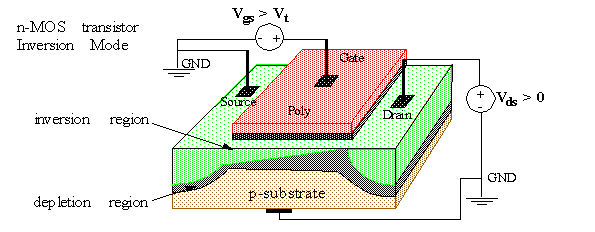
\includegraphics[width=\textwidth]{mos_transistor.png}
		\caption[Corte de transistor MOSFET]{Corte de transistor MOSFET\protect\footnotemark}
		\label{fig:mos_transistor.png}
	\end{figure}

	\footnotetext{Fuente: \url{http://ece-research.unm.edu/jimp/vlsi/slides/chap2_1.html} }
	
	Un transistor MOSFET es un tipo de transistor bipolar que se usa para amplificar y conmutar señales eléctricas dentro de un circuito. Se compone de cuatro entradas: fuente, puerta, drenador, y sustrato, que normalmente está conectado a la fuente. Cuando se aplica un voltaje en la puerta, se crea un canal en el medio semiconductor que permite el paso de corriente entre la fuente y el drenador. Podemos distinguir dos tipos de transistores MOS: los canal-n y los canal-p, dependiendo del dopaje del silicio usado en su fabricación. Los canal-n tienen un dopaje negativo en el silicio de la fuente y el drenador, que se consigue añadiendo impurezas de un elemento como fósforo, dejando electrones libres que actúan como portadores de carga. En el caso de los canal-p, se dopan con elementos como boro, que dejan huecos (ausencia de electrones en capas de valencia), y estos actúan como portadores de carga.
	
	Estos son los símbolos más usados para representar transistores MOS:
	
	\begin{figure}[h]
		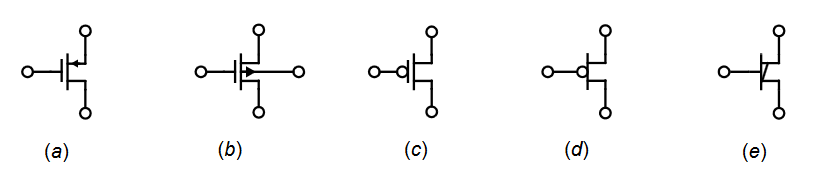
\includegraphics[width=\textwidth]{p-mos-symbol.png}
		\caption[Transistor MOS, canal-p]{Transistor MOS, canal-p\protect\footnotemark}
		\label{fig:p-mos-symbol.png}
	\end{figure}

	\footnotetext{Fuente: Analog Integrated Circuit Design\cite{aicd}}
	
	\begin{figure}[h]
		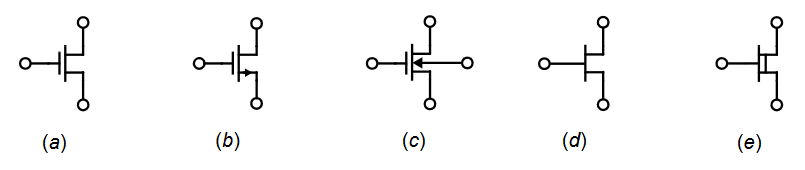
\includegraphics[width=\textwidth]{n-mos-symbol.png}
		\caption[Transistor MOS, canal-n]{Transistor MOS, canal-n\protect\footnotemark}
		\label{fig:n-mos-symbol.png}
	\end{figure}
	
	
	\footnotetext{Fuente: Analog Integrated Circuit Design\cite{aicd}}
	
	\section{Tecnología CMOS}
	
	La tecnología de fabricación CMOS\footnote{Complementary MOS} utiliza una combinación de transistores MOS de canal n y canal p para implementar las funciones de un microprocesador. Por ejemplo, un inversor (puerta lógica NOT) se consigue con la siguiente disposición:
	
	\begin{figure}[h]
		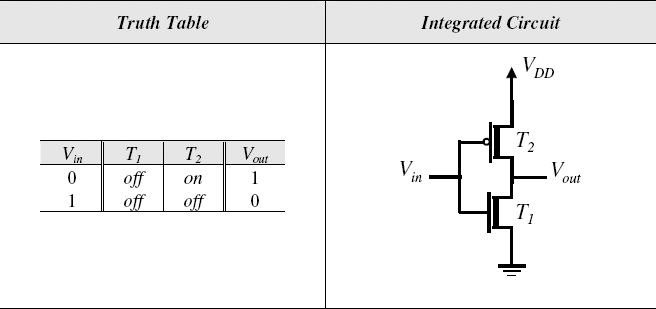
\includegraphics[width=\textwidth]{inverter_mos.jpg}
		\caption[Inversor CMOS]{Inversor CMOS\protect\footnotemark}
		\label{fig:inverter_mos.jpg}
	\end{figure}
	\footnotetext{Fuente: \url{https://www.oreilly.com/library/view/introduction-to-digital/9780470900550/chap5-sec008.html} }
	
	Los circuitos CMOS tienen un bajo consumo, tienen una buena resistencia al ruido, y son relativamente fáciles de diseñar. Es por esto que se ha convertido en la tecnología dominante en los microcircuitos.
	
	\section{Conversión analógico-digital}
	
	
	
	
	
\chapter{Métodos (?)}
\chapter{Conclusiones (?)}
\chapter{Entorno socioeconómico (?)}
\chapter{Presupuesto / planificación / proceso (?)}

%----------
%	BIBLIOGRAFÍA
%----------	

%\nocite{*} % Si quieres que aparezcan en la bibliogdrafía todos los documentos que la componen (también los que no estén citados en el texto) descomenta está lína

\clearpage

\addcontentsline{toc}{chapter}{Bibliografía}
\setquotestyle[english]{british} % Cambiamos el tipo de cita porque en el estilo IEEE se usan las comillas inglesas.
\printbibliography

%----------
%	ANEXOS
%----------	

% Si tu trabajo incluye anexos, puedes descomentar las siguientes líneas
%\chapter* {Anexo x}
%\pagenumbering{gobble} % Las páginas de los anexos no se numeran



\end{document}